%*************************************************************
\section{System Models and Assumptions}
\label{sec:systemModel}
%*************************************************************
\noindent {\bf The threat model.} This study is focused on system end-to-end security based on an adversarial perspective.  Call  $W_{DBaaS}$ the set of databases managed by a DBaaS:

\begin{equation}
\label{eq:DBaaS}
W_{DBaaS}=\Big \langle D_1,\dots, D_n \Big \rangle
\end{equation}
Each database $D_{i} ~, ~~ 1 \le i \le n$ consists  of an arbitrary number  $m$ of documents:

\begin{equation}
\label{eq:Database}
D_\imath = \big\{ d_1,\dots,d_m\big\}\\
\end{equation}
A document $d_{j}~,~~1 \le  j \le m$ includes an arbitrary number $l$ of key-value pairs $\langle key, value\rangle$: 

\begin{equation}
\label{eq:Document}
d_\jmath=\big\{ A_1,\dots, A_l\big\} 
\end{equation}

\noindent The function, $\Psi_{\epsilon}(D_i,D_j)$ in Equation \ref{eq:attributeCorrelation} is used to measure the information leakage $\mathcal{L}$ from any given pair of two databases $D_P$ and $D_Q$ as a result of cross-correlation:   

\begin{equation}
\label{eq:attributeCorrelation}
\begin{aligned}
\Psi (D_P, D_Q):
& \forall~d_p \in D_P ~\land~ \forall~ d_q \in D_Q ~~if~~ (\mu(d_p,d_q)==True) \implies \mathcal{L}=\Delta(d_p, ~d_q) 
\end{aligned}
\end{equation}

Where $\mathcal{L}$ is set of the leaked attributes and the operator $\Delta$ is the symmetric difference operator which is the union of all attributes from both documents without the intersection, and '\textbackslash' ~ is relative complement. The $\Delta$ can be restated as $\Delta(d_p, ~d_q) =(d_p\setminus d_q)\cup (d_q\setminus d_p)$.

\noindent The feasibility function $\mu$ in Equation \ref{eq:attributeCorrelation} determines if a given pair of documents can be merged according the type of shared attribute. The $\mu$ function is outlined in Equation \ref{eq:muFunction}.


\begin{equation}
\label{eq:muFunction}
\begin{aligned}
& \mu(d_p,d_q)= \begin{cases}
&\textbf{True} \\
&iff \quad \exists A_r \in d_p ~ \land ~\exists A_s \in d_q ~ \mid [(A_r.key==A_s.key) \land (A_r.value==A_s.value)]\\
\noalign{\text{Such that $A_r, A_s$ are indentifier attributes of $d_p, d_p$}}
&\textbf{False} \qquad Otherwise
\end{cases}
\end{aligned}
\end{equation}

An adversarial threat analysis starts with thinking like an attacker and continues to prepare the corresponding countermeasure. Two classes of threats, external and internal attackers are identified by the model. External attacks can be conducted after obtaining unauthorized access to data or by using tools to monitor the communication between the clients and the cloud servers. External attackers face a more complex task since they need to bypass firewalls, intrusion detection systems, and other protection mechanisms.


Insider attacks can be conducted by the employees and the contractors of large data centers with access to the software, the hardware, and the data. A malicious insider could leak highly sensitive documents or use it for nefarious activities. There is also the risk of an intruder gaining the same level of access using the credentials of a legitimate employee. An insider can bypass internal protection mechanism and pose serious risks to data \textit{confidentiality}, \textit{integrity} and \textit{inference} violations. The list of possible insider attacker actions are denoted as $A=\{C, I,\Psi \}$ respectively.

The risk factors and the corresponding solutions as well as the advantages and disadvantages of the proposed solution are summarized in Figure\ref{fig:MIriskFactors}.

\begin{figure}[H]
\centering
\resizebox{0.9\textwidth}{!}{\begin{tikzpicture}[
block/.style={rectangle,draw,fill=gray!20,text width=9em,text centered,rounded corners,minimum height=4em,node distance=0.4cm,auto},
line/.style={draw,-latex',node distance= 2cm,auto}]

\node [block] (a) {Confidentiality violation};
\node [block, below=of a] (b) {Integrity violation};
\node [block, below=of b] (c) {Information leakage};

\node [block, right=of a] (sa) {Cryptosystems:\\AHOM, OPE, \\DET, RND };
\node [block, right=of b] (sb) { Query verification};
\node [block, right=of c] (sc) {1-Query tracking\\2-Selective insertion of disinformation};

\node [block, right=of sa] (aa) {1-Confidentiality\\2-Full control\\ over data};
\node [block, right=of sb] (ab) {Data authenticity};
\node [block, right=of sc] (ac) {1-Leakage limitation\\ 2-Indistinguishable info. and disinfo};

\node [block, right=of aa] (da) {1-Limited operations\\2-Computation cost};
\node [block, right=of ab] (db) {1-Computation cost\\2-Token overhead};
\node [block, right=of ac] (dc) {1-Data overhead\\2-Filter \& verification cost};

\path [line] (a) -- node {}(sa);
\path [line] (b) -- node {}(sb);
\path [line] (c) -- node {}(sc);


\path [line] (sa) -- node {}(aa);
\path [line] (sb) -- node {}(ab);
\path [line] (sc) -- node {}(ac);

\path [line] (aa) -- node {}(da);
\path [line] (ab) -- node {}(db);
\path [line] (ac) -- node {}(dc);

\node[label={\large Risk factor}]  at (-0.15,1) {};
\node[label={\large Mitigation}]  at (4.0,1) {};
\node[label={\large Advantage}]  at (8.5,1) {};
\node[label={\large Disadvantage}]  at (13.0,1) {};
\end{tikzpicture}
}
\caption{Risk factors posed by malicious insiders; the advantages and disadvantages of proposed responses.}
\label{fig:MIriskFactors}
\end{figure}

\noindent An insider has read/write access in the data warehouse and activity log files and could target sensitive information about entity $\bm{\varepsilon}$ stored as a set of $\langle key, value \rangle$ pair(s). The attacker has one initial document stored in database $D_i$ and his goal is to obtain sensitive attributes of $\varepsilon$. 

\smallskip

\noindent {\it Confidentiality violation risk.} The attacker misuses her existing privileges to gain further access to sensitive information without any trace of intrusion. Such attacks are very hard to detect because the attacker is authorized to carry out the operation used for intrusion. 

\underline{Mitigation:} Cryptographic schemes can be used to encrypt data before cloud outsourcing. Processing encrypted data without decryption restrict the selection of cryptographic schemes selection.

An insider attacker can extract an encrypted sensitive attribute $\hat{A}=\langle E_k(key), E_k(value) \rangle$ related to an entity of interest $\bm{\varepsilon}$ stored in database $D_i$ by iteratively calling the cross-correlation function $\Psi (D_i, D_j), \forall j \in [1, n]$. Two databases $D_i$ and $D_j$ may initially not share any documents, but they may be linked by cross-correlation each one of them has with other databases.

\noindent {\it Integrity violation (active attack) risk.} Integrity verification ensures that data is only modified by an authorized user and identifies integrity violation done by an intruder. Query integrity verification is a tamper-resistant algorithm built on Message Authentication Codes (MAC). We append a new attribute named \emph{eTag} to each document containing a keyed hash value of the entire document. The data owner generates the augmented attribute $\langle eTag, E_k(d_i)\rangle$ for any document $d_i$ including disinformation. 
According to semantic security principle, the original and fake documents should be indistinguishable. Thus, the same procedure for generation of eTag conducted for the disinformation documents. In particular, a sensitive attribute can be seen as an equivalent class for $\mathcal{V}$ attributes that have diverse value for attributes to prevent disclosure. Finally, the attributes of real and fake documents are encrypted according to the security plan and forwarded to the DBaaS in the cloud. Figure \ref{fig:eTagAttribute} illustrates the process of eTag attribute production for the documents.

%Figure eTag
\begin{figure}[H]
\centering
\resizebox{0.8\textwidth}{!}{\tikzset{
table nodes/.style={
rectangle,
draw=black,
align=center,
minimum height=6mm,
text depth=0.5ex,
text height=2ex,
inner xsep=0pt,
outer sep=0pt
},      
table/.style={
matrix of nodes,
row sep=-\pgflinewidth,
column sep=-\pgflinewidth,
nodes={
    table nodes
},
execute at empty cell={\node[draw=none]{};}
}
}
\tikzstyle{doc}=[%
draw,
thick,
align=left,
color=black,
shape=document,
minimum width=8mm,
minimum height=5mm,
]
\begin{tikzpicture}[scale=0.8,align=left]
\node (Info)[doc,fill=green!20, fill opacity=0.5,text opacity=1] {
\begin{tikzpicture}
\node[label={\textbf{Info doc}}] (A) at (-10,0) {};
\matrix (B) [table,text width=15mm,below =-4mm of A, ampersand replacement=\&]
{
$Key_1$     \& $Value_1$\\
...         \& ...\\
$Key_n$     \& $Value_n$\\
};
\end{tikzpicture}
};
\node (DisInfo)[doc,below=2mm  of Info,fill=red!20, fill opacity=0.4,text opacity=1] {
\begin{tikzpicture}
\node[label={\textbf{Disinfo doc}}, color=black] (A) at (0,0) {};
\matrix (B) [table,text width=15mm,below =-5mm of A,  ampersand replacement=\&]
{
$Key_1$     \& $Value_1$\\
...         \& ...\\
$Key_n$     \& $Value_n$\\
};
%\node [rectangle,text width=0.1cm,minimum height=0em,right= of B] (C) {};
\end{tikzpicture}
};
\node[box1, fill=gray!20, fill opacity=0.3,text opacity=1, every text node part/.style={align=left}] (Enc) at (7,-1) {{\normalsize \\$Digest = Hash\{Document\}$\\ $eTag:\bm{E_k\{Token\Vert Digest\}}$};

\node[box1, fill=gray!20, fill opacity=0.4,text opacity=1, every text node part/.style={align=left}] (eTag) at (14.5,-1) {{\underline{Encryption}}\\ \\{ $E_k(Key_1):E_k(Value_1)$} \\.. \\$E_k(Key_n):E_k(Value_n)$};
\node (EncDoc)[doc,below=0.5  of eTag,fill=white, fill opacity=0.1,text opacity=1] {
\begin{tikzpicture}
\node[label={\textbf{Encrypted doc}}, color=black] (ED)  {};
\matrix (B) [table,text width=22mm,below =-5mm of ED, ampersand replacement=\&]
{
$\color{red} \bm{eTag}$ \&$\color{red}\bm{value}$\\
$E_k(Key_1)$     \& $E_k(Value_1)$\\
...         \& ...\\
$E_k(Key_n)$     \&$E_k(Value_n)$\\
};
\end{tikzpicture}
};

\node (EncDoc2)[doc,fill=white,fill opacity=1.0,text opacity=1]  at (13.5,-7.0) {
\begin{tikzpicture}
\node[label={\textbf{Encrypted doc}}, color=black] (ED)  {};
\matrix (B) [table,text width=22mm,below =-5mm of ED, ampersand replacement=\&]
{
$\color{red} \bm{eTag}$ \&$\color{red}\bm{value}$\\
$E_k(Key_1)$     \&$E_k(Value_1)$\\
...         \& ...\\
$E_k(Key_n)$\&$E_k(Value_n)$\\
};
\end{tikzpicture}
};
\draw[->, >=latex, black!70, line width=4pt,rotate=-90]   (DisInfo) to node[black]{} (Enc) ;
\draw[->, >=latex, black!70, line width=4pt,rotate=-90]   (Info) to node[black]{} (Enc) ;
\draw[->, >=latex, black!70, line width=4pt,rotate=-90]   (Enc) to node[black]{} (eTag) ;
\draw[->, >=latex, black!70, line width=4pt,rotate=-90]   (eTag) to node[black]{} (EncDoc) ;

\end{tikzpicture}}
\caption{The high level description of \textit{eTag} attribute production.}
\label{fig:eTagAttribute}
\end{figure}

To minimize the information leakage, the attributes which are the lowest level of data granularity, data are encrypted with RND encryption. Equation \ref{eq:NonDeterminsticEncryption} outlines RND (non-deterministic) encryption function constructed from a deterministic one. First we associate a unique fixed length random number $r$, with each document. With application of eTag, the risk of active attack and unauthorized modification by third party is detectable in the verification phase in the proxy.


\begin{equation}
\label{eq:NonDeterminsticEncryption}
\begin{aligned}
& E_k (x) = E^{\prime}_k (x \left\lvert \right\rvert r) \\ 
\end{aligned}
\end{equation}
Where: $k$ is the encryption key; $E^{\prime}$ is a DET encryption; $r$ is a random number.\\


\medskip

\noindent {\it Information leakage risk.} Encrypted databases are prone to information leakage, for instance deterministic and OPE cryptographic schemes always leak frequency and the order of plaintext data respectively. Subsequently, with a simple frequency analysis or sorting attack, insider attackers are able to obtain sensitive information. Later on, with an inference attack they combine leaked data with information in the other databases in the same cloud DBaaS or a public domain to hack the database.
 
The probability for one attribute to be extracted from $n$ databases with success probability p for each database is given by Equation \ref{oneSuccess}. Nevertheless, appending $\mathcal{V}$ disinformation documents per each correlated document creates $\mathcal{V}$ value from a sensitive attribute. Ultimately, the result is a full tree-like structure with branch factor $\mathcal{V}+1$  which requires exponential computation to be extracted. Equation \ref{numberOfNodes} displays the number of values for a sensitive attribute after insertion of disinformation. As it can be seen, the number of branches is proportional to height $h$.

\begin{equation}
\label{oneSuccess}
f(1;n,p) = n\times p\times(1-p)^{n-1}
\end{equation}

\begin{equation}
\label{numberOfNodes}
N = 1+\mathcal{V}+ \mathcal{V}^2+ \dots + \mathcal{V}^h= \frac{\mathcal{V}^{h+1}-1}{\mathcal{V}-1}.
\end{equation}

Eventually, the new probability distribution function for extraction of $k$ attributes from $n$ databases which are diluted with $\mathcal{V}$ disinformation is displayed in Equation \ref{attributeFromDilutedDB}.
\begin{equation}
\label{attributeFromDilutedDB}
f(k;n,p) = \prod_{i=0}^{\mathcal{V}} {{N} \choose {k}}p^{\frac{k}{i}}(1-p)^{N-k}
\end{equation}

\medskip

\noindent {\it Query integrity verification.} The augmented eTag attribute is useful in two ways, including data and query integrity verification. Having eTag attribute in place makes the disinformation documents identifiable, thus, the proxy filters out them from the query response. The proxy decrypts eTag value with the decryption key and verifies the tag of original documents from the query response and filters out the disinformation documents. The MAC are used to protect against any unauthorized modifications of documents. With the mechanism of digital signature that implemented in eTag, the proxy verifies the authenticity of whole document with recalculation of document digest and verification with the digest. The digital signature of the documents adds a small overhead to the documents, however it guarantees the document never gets modified by cloud insiders. Intuitively, eTag is not involved in a query processing and this attribute will be used for the internal structure for providing integrity of data store. The verification process grantees the authenticity and integrity of documents as presented in Equation \ref{eTagVerification}.
\begin{equation}
\label{eTagVerification}
\begin{aligned}
&Verification: \\
&eTag^{'}= MAC_k(document); \quad \begin{cases}
&if (eTag==eTag^{'}) \implies Document~is~valid.\\
&else~ Document~ is~ invalid. 
\end{cases}
\end{aligned}
\end{equation}


The crypto-hash functions are building blocks of the introduced query integrity verification algorithm, and therefore, having an efficient hash function leads to low latency integrity verification. We examined the performance of four popular hash functions according to the variety of document size. The result is displayed in Figure \ref{fig:hashPerformance}. Considering the performance and security metrics, we select \emph{SHA1} over other hash functions including MD5, RIPEMD and SHA256 to be used in eTag algorithm. As it can be observed from Figure \ref{fig:hashPerformance}, the reason of selection of SHA1 is its high performance (speed) at different input documents sizes.

%Figure
\begin{figure}[H]
\centering
\resizebox{0.6\textwidth}{!}{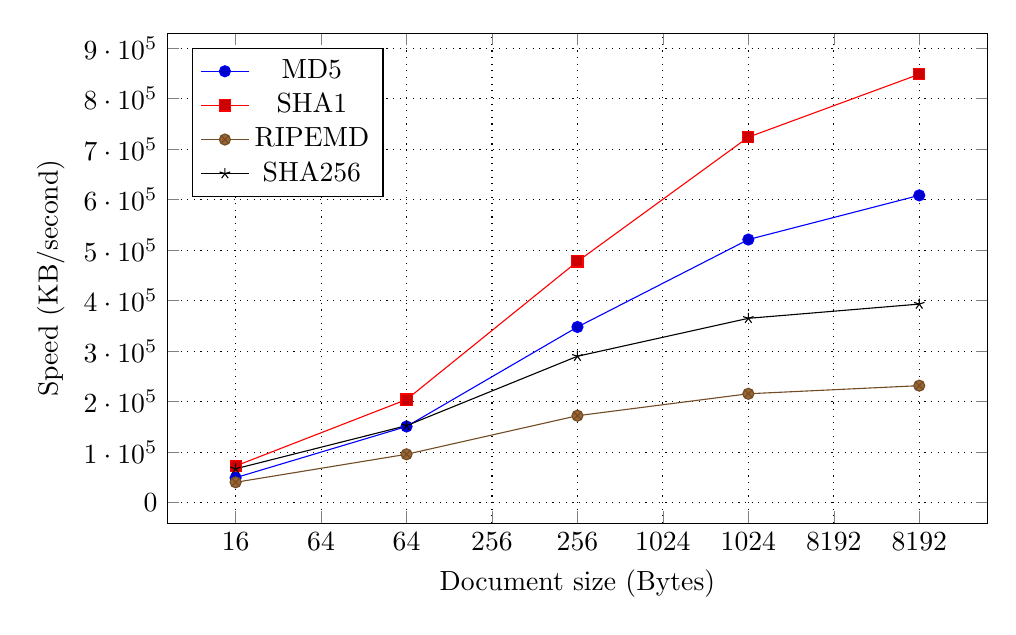
\begin{tikzpicture}
\begin{axis}[legend style={at={(0,0)},anchor=west,at={(axis description cs:1.05,0.45)}},    title={},
ytick={0,100000,200000,300000,400000,500000,600000,700000,800000,900000},
symbolic x coords={16,64,256,1024,8192},
%ytick=data,
xlabel={Document size (Bytes)},
ylabel={Speed (KB/second)},
scaled y ticks=false, 
compat=newest, %Better
legend pos=north west,
%axis background/.style={fill,bottom color=gray!50,top color=white},
grid=major,
height=7.8cm,width=12cm,
grid style={dotted,black}
]
\addplot+ coordinates {
	(16,49292.32)      %16
	(64,150689.13)     %64
	(256,347740.76)    %256
	(1024,520933.03)   %1024
	(8192,608428.03)   %8192
};
\addlegendentry{MD5}
\addplot+ coordinates {
	(16,72490.62)      %16
	(64,204046.66)     %64
	(256,477543.25)    %256
	(1024,723760.47)   %1024
	(8192,848322.56)   %8192
};
\addlegendentry{SHA1}
\addplot+ coordinates {
	(16,40183.96)      %16
	(64,95633.13)      %64
	(256,172034.90)    %256
	(1024,215498.41)   %1024 
	(8192,231541.42)   %8192
};
\addlegendentry{RIPEMD}
\addplot+ coordinates {
	(16,66921.74)      %16
	(64,152366.29)     %64
	(256,289791.49)    %256
	(1024,364940.63)   %1024 
	(8192,393106.77)   %8192
};
\addlegendentry{SHA256}
\end{axis}
\end{tikzpicture}}
\caption{Performance of four popular cryptographic hash functions in respect to document size.}
\label{fig:hashPerformance}
\end{figure}


The dynamic nature of a dataset as a persistent storage necessitate to have basic operations to create, read, update and delete (known as CRUD). The augmented dataset (with disinformation documents), naturally are subjected to CRUD operations. The create and read operations act on the augmented dataset in a similar way to a normal dataset, while the update/delete operations on the original documents should be projected on the corresponding disinformation documents. For the performance purpose, the update/delete operations on the related disinformation documents, can be processed immediately or in lazy fashion, postponed to the next period of the data analysis. Furthermore, the garbage collector service, run by the proxy, can be developed to delete any unrelated disinformation from the dataset. The design and development of such a service is beyond the scope of the current work. 

%We propose \emph{Selective Disinformation Document Padding (SPDP)} to hinder information extraction, while avoiding overhead of disinformation document padding. SPDP uses metrics such as precision and recall, as well as statistical analytics to periodically probe the dataset for explicit and/or implicit cross-correlations between data elements. Thereafter, the detected leakage is compared to the maximum acceptable level of leakage. If the result exceeds the maximum level established by the data owner, the SPDP mechanism generates a number of fake documents to be inserted into the dataset. The number of generated disinformation documents depends on the significance of the leakage metrics.